\documentclass[article]{jss}

%%uncomment line below for double-spacing
\linespread{1}
\setlength{\parskip}{0.5cm}%

%%%%%%%%%%%%%%%%%%%%%%%%%%%%%%
%% declarations for jss.cls %%%%%%%%%%%%%%%%%%%%%%%%%%%%%%%%%%%%%%%%%%
%%%%%%%%%%%%%%%%%%%%%%%%%%%%%%

%% almost as usual
\author{Joseph Kelly\\Harvard University \And 
             Hyungsuk Tak\\Harvard University\And
             Carl Morris\\ Harvard University}
\title{\pkg{Rgbp}: An R Package for Gaussian, Poisson, and Binomial Hierarchical Modeling}

%% for pretty printing and a nice hypersummary also set:
\Plainauthor{Joseph Kelly, Carl Morris, Hyungsuk Tak} %% comma-separated
\Plaintitle{Rgbp: An R Package for Hierarchical modeling and Method Checking} %% without formatting

%% an abstract and keywords
\Abstract{
\pkg{Rgbp} is an R package that utilizes approximate Bayesian machinery to provide a method of estimating two-level hierarchical models for Gaussian, Poisson, and Binomial data in a fast and computationally efficient manner. The main products of this package are point and interval estimates for the true parameters, whose good frequency properties can be validated via its repeated sampling procedure called ``frequency method checking."  It is found that such Bayesian-frequentist reconciliation allows \pkg{Rgbp} to have attributes desirable from both perspectives, working well in small samples and yielding good coverage probabilities for its interval estimates.}
\Keywords{multilevel model, conjugate hierarchical generalized linear models, frequency method checking, coverage probability, shrinkage}
\Plainkeywords{keywords, comma-separated, not capitalized, r} %% without formatting
%% at least one keyword must be supplied

%% publication information
%% NOTE: Typically, this can be left commented and will be filled out by the technical editor
%% \Volume{50}
%% \Issue{9}
%% \Month{June}
%% \Year{2012}
%% \Submitdate{2012-06-04}
%% \Acceptdate{2012-06-04}

%% The address of (at least) one author should be given
%% in the following format:
\Address{
  Joseph Kelly\\
  Department of Statistics\\
  Harvard University\\
  1 Oxford Street, Cambridge, MA\\
  E-mail: \email{kelly2@fas.harvard.edu}\\
  URL: \url{http://www.people.fas.harvard.edu/~kelly2/}\\

  Hyungsuk Tak\\
  Department of Statistics\\
  Harvard University\\
  1 Oxford Street, Cambridge, MA\\
  E-mail: \email{hyungsuk.tak@gmail.com}\\

  Carl Morris\\
  Department of Statistics\\
  Harvard University\\
  1 Oxford Street, Cambridge, MA\\
  E-mail: \email{morris@fas.harvard.edu}\\
}

%% It is also possible to add a telephone and fax number
%% before the e-mail in the following format:
%% Telephone: +43/512/507-7103
%% Fax: +43/512/507-2851

%% for those who use Sweave please include the following line (with % symbols):
%% need no \usepackage{Sweave.sty}

%% end of declarations %%%%%%%%%%%%%%%%%%%%%%%%%%%%%%%%%%%%%%%%%%%%%%%

\begin{document}
%% include your article here, just as usual
%% Note that you should use the \pkg{}, \proglang{} and \code{} commands.

\section[introduction]{Introduction}
%% Note: If there is markup in \(sub)section, then it has to be escape as above.
\pkg{Rgbp} is an R package for estimating and validating a two-level model, also called conjugate hierarchical generalized linear model \citep{hglm2006, hglm2010} or called a conditionally independent hierarchical model \citep{1989}, producing point and interval estimates of the true parameters. The estimation procedure utilizes approximate Bayesian machinery and the validation involves checking frequency properties of the procedure via repeated sampling (which we call ``frequency method checking"). It is found that even in small samples our procedure yields good frequency properties in comparison to other methods such as Maximum Likelihood Estimation (MLE). 

This package will be useful for frequentists and Bayesians alike. Bayesians are able to use the package to see results for a non-informative reference prior before and after constructing their own Bayesian hierarchical model. Frequentists will have a procedure that meets or exceeds their confidence specification and repeated sampling.


%\section[Feasible Data Types]{Three Feasible Types of Data }
%\pkg{Rgbp} is intended to fit a model where two levels of structure are assumed (unit and group levels). The model can be characterized by the distributional family assumed for the group level data and in the case of \pkg{Rgbp} this will be either the Normal, Poisson, or Binomial distribution. In this section, we will introduce three specific types of feasible data sets that illustrate this fact.

%\subsection{Normal: 8 Schools} \label{8schooldata}
%The Education Testing Service (ETS) conducted randomized experiments in eight separate schools (group) to test whether students (unit) SAT scores are effected by coaching. The dataset contains the estimated coaching effects on SAT scores ($y_{j}, j=1, \ldots, 8$) and standard errors ($se_{j}, j=1, \ldots, 8$) of the eight schools \citep{1981}.
%\begin{CodeChunk}
%\begin{CodeInput}
%R> y  <- c(12, -3, 28,  7,  1,  8, 18, -1)
%R> se <- c(18, 16, 15, 11, 11, 10, 10,  9)
%\end{CodeInput}
%\end{CodeChunk}

%Due to the nature of the test each school's coaching effect has an approximately Normal sampling distribution with known sampling variance, \emph{i.e.}, standard error of each school is assumed to be known or to be accurately estimated. So, it is reasonable to think that each school-level coaching effect is distributed as an independent Normal distribution given the unknown mean $\mu_{j}$ and known standard error:  $y_{j}\vert\mu_{j}\stackrel{ind}{\sim} \textrm{Normal}(\mu_{j}, se^{2}_{j}),~ j=1, \ldots, 8$. \pkg{Rgbp} includes this data set and can be called by the command `\code{data(schools)}' on \proglang{R}.

%\subsection{Poisson: 31 Hospitals}
%The following data are from medical profiling evaluations for Coronary Artery Bypass Graft (CABG) surgeries of 31 New York hospitals conducted in 1992 \citep{2012}. It comprises of the number of deaths within a month of CABG surgeries in each hospital ($z_{j},~j=1, \ldots, 31$) and the total number of patients receiving CABG surgeries (case load) in each hospital ($n_{j},~j=1, \ldots, 31$). The following code is an example of input based on the last ten hospital data.
%\begin{CodeChunk}
%\begin{CodeInput}
%R> z <- c( 14,   9,  15,  13,  35,  26,  25,  20,   35,   27)
%R> n <- c(593, 602, 629, 636, 729, 849, 914, 940, 1193, 1340)
%\end{CodeInput}
%\end{CodeChunk}
%Considering the type of data, it is reasonable to assume the number of deaths in each hospital follow independent Poisson distributions given an unknown true rate parameter $\lambda_{j}$: $z_{j}\vert \lambda_{j}\stackrel{ind}{\sim} \textrm{Poisson}(n_{j}\lambda_{j})$, $j=1, \ldots, 31,$ where, for each $j$, $n_{j}$ can be interpreted as an exposure (not necessarily an integer) and $\lambda_{j}$ as the true death rate per exposure. This data set is also included in the package and can be called by `\code{data(hospital)}' on \proglang{R}.

%\subsection{Binomial: 18 Baseball Hitters}
%The following dataset contains information on the batting averages of 18 major league baseball players through their first 45 official at-bats of the 1970 season \citep{1975}. In addition one covariate relating to the position each player was playing was observed and for illustrative purposes, we transform this variable into a binary indicator (1 if a player was an outfielder and 0 otherwise).
%\begin{CodeChunk}
%\begin{CodeInput}
%R> z <- c(18, 17, 16, 15, 14, 14, 13, 12, 11, 11, 10, 10, 10, 10, 10,  9,  %8,  7)
%R> n <- c(45, 45, 45, 45, 45, 45, 45, 45, 45, 45, 45, 45, 45, 45, 45, 45, %45, 45)
%R> x <- c( 1,  1,  1,  1,  1,  0,  0,  0,  0,  1,  0,  0,  0,  1,  1,  0,  0,  0) 
%\end{CodeInput}
%\end{CodeChunk}
%The data indicate that independent Binomial distribution is appropriate for each player's number of hits among 45 at-bats conditioning on the unknown true batting average $p_{j}$: $z_{j}\vert p_{j}\stackrel{ind}{\sim} \textrm{Binomial}(n_{j}, p_{j}), ~j=1, \ldots, 18$. This data set is also a part of the package and can be called on \proglang{R} by `\code{data(baseball)}'.

\section[Hierarchical Structure]{Hierarchical Structure} \label{hierarchical}
A two-level or multilevel model is a powerful tool for exploring the hierarchical structure in data. For example, we can imagine that there exists a district-level hierarchy (bigger population) for observed school-level data, or a state-level hierarchy for observed hospital-level data in a certain state. 



\code{gbp}, one of the functions in \pkg{Rgbp}, fits such a hierarchical model whose first-level has distributions of observed data and whose second-level has conjugate distributions on the first-level parameters. The \code{gbp} function allows users to choose one of three types of hierarchical models, namely Normal-Normal, Poisson-Gamma, and Binomial-Beta. 
 
\subsection[Normal-Normal]{Normal-Normal (``g''=Gaussian data)}
The following is the general Normal-Normal hierarchical model assumed by \code{gbp}. For reference,  $V_{j}~(\equiv \sigma^{2}/n_{j})$ below is assumed to be known or to be accurately estimated, and subscript \emph{j} indicates the \emph{j}-th group among \emph{k} groups in the dataset.
\begin{equation}\label{normalobs}
y_{j}\vert \mu_{j} \stackrel{ind}{\sim}\textrm{Normal}(\mu_{j}, V_{j}),
\end{equation}
\begin{equation}\label{normalprior}
\mu_{j}\vert \beta, A\stackrel{ind}{\sim}\textrm{Normal}(\mu_{0j}, A),
\end{equation}

where $\mu_{0j} = x^{T}_{j} \mathbf{\beta}_{(m\times1)}=\beta_{0}+\beta_{1}x_{1, j} + \cdots + \beta_{m-1}x_{m-1, j}$, $j=1, \ldots k$ and $m$ is the number of regression coefficients including an intercept term. The notation $x_{j}^{T}=(1, x_{1, j}, x_{2, j}, \ldots, x_{m-1, j})$ represents the $j$-th group's $m\times 1$ covariate vector whose first element is 1 for the intercept term of regression coefficients. Both $\mathbf{\beta}_{(m\times1)}$ and the second-level variance $A$ are unknown. Note that if there is no covariate then $x_{j}=1$ just for an intercept term ($m=1$) and so $\mu_{0j}=\mu_{0}=\beta_{0}$ for all $j$, resulting in an exchangeable prior distribution. For reference, a parameter with a zero subscript, such as $\mu_{0j}$, represents a mean parameter of the prior (second-level) distribution, \emph{i.e.}, a prior mean. Based on this conjugate prior distribution it is easy to derive the corresponding posterior distribution
\begin{equation} \label{normalpost}
\mu_{j}\vert \textbf{y}, \beta, A \stackrel{ind}{\sim}\textrm{Normal}(~(1-B_{j})y_{j} + B_{j}\mu_{0j},~(1-B_{j})V_{j}~),
\end{equation}
where $B_{j}\equiv V_{j}/(V_{j} + A),~j=1, \ldots, k$, are called shrinkages.

\subsection[Poisson-Gamma]{Poisson-Gamma (``p''=Poisson data)}\label{poissonsubsec}
\code{gbp} is also able to build a Poisson-Gamma hierarchical model. Note that a constant, $1/r$, multiplied to the Gamma distribution below is a scale and a square bracket [, ] below indicates [mean, variance] of a distribution. For notational consistency, let's define $y_{j}\equiv z_{j} / n_{j}$ as the unbiased estimate of $\lambda_{j}$ for the $j$-th group.
\begin{equation}
z_{j}\vert \lambda_{j} \stackrel{ind}{\sim}\textrm{Poisson}(n_{j}\lambda_{j}),
\end{equation}
\begin{equation}\label{gammaprior}
\lambda_{j}\vert \beta, r\stackrel{ind}{\sim}\frac{1}{r}\textrm{Gamma}(r\lambda_{0j})\sim \textrm{Gamma} \left[\lambda_{0j}, ~\frac{\lambda_{0j}}{r} \right],
\end{equation}

where $\log(\lambda_{0j}) =x_{j}'\beta$, $j=1, \ldots, k$, with two unknown hyper-parameters, $\beta$ and $r$. The posterior distribution of this Poisson-Gamma model given these hyper-parameters is
\begin{equation} \label{gammapost}
\lambda_{j}\vert \textbf{y}, \beta, r \stackrel{ind}{\sim}\frac{1}{r + n_{j}}\textrm{Gamma}(r\lambda_{0j} + n_{j}y_{j})\sim\textrm{Gamma} \left[\lambda^{\ast}_{j},~\frac{\lambda^{\ast}_{j}}{r+n_{j}} \right],
\end{equation}

where $\lambda^{\ast}_{j} \equiv (1-B_{j})y_{j} + B_{j}\lambda_{0j}$ and   $B_{j}\equiv r / (r+n_{j})$ for $j=1, \ldots, k$. 


Note that the variance in (\ref{gammaprior}) is linear in the mean, whereas a slightly different Poisson-Gamma specification \citep{1997} has been used elsewhere e.g. that makes the variance in (\ref{gammaprior}) quadratic.

\subsection[Binomial-Beta]{Binomial-Beta (``b''=Binomial data)}
Binomial-Beta hierarchical model is the last model that \code{gbp} can fit. Again, a square bracket below indicates [mean, variance] of a distribution.
\begin{equation}
z_{j} \vert p_{j}\stackrel{ind}{\sim}\textrm{Binomial}(n_{j}, ~p_{j}),
\end{equation}
\begin{equation}
p_{j} \vert \beta, r\stackrel{ind}{\sim}\textrm{Beta}(rp_{0j},~ r(1-p_{0j}))\sim \textrm{Beta} \left[p_{0j}, ~\frac{p_{0j}(1-p_{0j})}{r + 1} \right],
\end{equation}

where $\log(\frac{p_{0j}}{1-p_{0j}}) =x_{j}'\beta, ~j=1, \ldots, k$ and $\beta$ and $r$ are two unknown hyper-parameters. Then corresponding posterior distribution given  $\beta$ and $r$ is
\begin{equation} \label{betapost}
p_{j}\vert \textbf{y}, \beta, r \stackrel{ind}{\sim}\textrm{Beta}(rp_{0j}+n_{j}y_{j},~r(1-p_{0j})+n_{j}(1-y_{j}))\sim\textrm{Beta}\bigg[p^{\ast}_{j},~ \frac{p^{\ast}_{j}(1-p^{\ast}_{j})}{r+n_{j}+1}\bigg],
\end{equation}
where $p^{\ast}_{j}\equiv(1-B_{j})y_{j}+B_{j}p_{0j}$, $B_{j}\equiv r/ (r+n_{j})$, and $y_{j}\equiv z_{j} / n_{j}$, $j=1,\ldots,k$.


\subsection[Hyper-prior Distribution]{Hyper-prior Distribution}
A hyper-prior distribution is a distribution assigned to the second-level parameters. With the goal of objectivity in mind our choice for hyper-priors with \code{gbp} assumes the following non-informative hyper-prior distributions:
\begin{equation}
\beta \sim \textrm{Uniform on}~ \mathbf{R}^{m}~~\textrm{and}~~A \sim \textrm{Uniform}(0, \infty) ~~(\textrm{or} ~\frac{1}{r}\sim \textrm{Uniform}(0, \infty)),
\end{equation}

where $m$ is the number of regression coefficients. As for $\beta$, the flat non-informative distribution above is a common choice. In the Gaussian case, the flat prior distribution on the second-level variance $A$ is chosen to produce good repeated sampling properties for point and interval estimates of the true parameters $\{\mu_{j}\}$, and to have its posterior propriety when $k\ge m+3$ \citep{2011}. In the other two cases, Poisson and Binomial, the distribution of $\frac{1}{r}$ induces the same improper prior distribution on shrinkages ($B_{j}$) as does $A$ with Uniform($0, \infty$) for the Gaussian. We will show the efficiency of this assignment  in the examples in section 5.



\section[Estimation]{Estimation}

\subsection[Shrinkage Estimation]{Shrinkage Estimation}
Estimating the shrinkage factors ($B_1, \ldots, B_k$) is the key estimation problem with the hierarchical models \code{gbp} assumes. As we can see in (\ref{normalpost}), (\ref{gammapost}), and (\ref{betapost}), the posterior means are a linear function of the shrinkage factors ($B_{j}$) and the posterior variances are linear (Gaussian), quadratic (Poisson), and  approximately cubic (Binomial) functions of $B_{j}$. A natural method then to estimate $E(\mu_{j}\vert \textbf{y})$ and $Var(\mu_{j}\vert \textbf{y})$ is to first estimate the shrinkage factors.

\subsection[ADM]{Approximation via Adjustment for Density Maximization}\label{ADM}
It is noted that the shrinkage factors ($B_1, \ldots B_k$) are a function of the second-level variance component, \emph{i.e.}, $B_{j}\equiv V_{j}/(V_{j}+A)=B_{j}(A)$ for Gaussian and $B_{j}\equiv r/(r+n_{j})=B_{j}(r)$ for Poisson and Binomial models. A common approach to approximate the distribution of $B_{j}$ is to find its MLE $\hat{B}_{j}(\hat{A}_{MLE})$ (or  $\hat{B}_{j}(\hat{r}_{MLE})$) and to use its asymptotic Normality. But its asymptotic Gaussian distribution is defined on $(-\infty, \infty)$ whereas $B_{j}$ is bounded between 0 and 1, and MLE can result in estimates lying on the boundary of the parameter space.

To continue with a maximization-based estimation procedure but to steer clear of aforementioned boundary issues we make use of adjustment for density maximization (ADM) \citep{carl1988, 1997, 2011}. For our purposes we approximate the posterior distribution of a shrinkage factor with a Beta distribution, which allows us to finally obtain estimates of the posterior moments, \emph{i.e.}  of $E(B_{j}\vert\textbf{y})$ and $Var(B_{j}\vert\textbf{y})$, where the notation $\textbf{y}$ represents observed data, without the boundary issues that MLE encounters. See \cite{2011}.

\subsection[Posterior Moment Estimation]{Posterior Moment Estimation}

Using the posterior mean and variance estimates of $B_{j}$, \pkg{Rgbp} estimates the posterior mean and variance of true parameters given only the data ($\textbf{y}$). Taking the Normal-Normal model as an example, it estimates $E(\mu_{j}\vert \textbf{y})$ and $Var(\mu_{j}\vert \textbf{y})$ by the following identities
\begin{eqnarray}
E(\mu_{j}\vert \textbf{y}) & = & E(E(\mu_{j}\vert \textbf{y}, \beta, A)\vert \textbf{y}), \\
Var(\mu_{j}\vert \textbf{y}) & = & E(Var(\mu_{j}\vert \textbf{y}, \beta, A)\vert \textbf{y})+Var(E(\mu_{j}\vert \textbf{y}, \beta, A)\vert \textbf{y}),
\end{eqnarray}  
where both $E(\mu_{j}\vert \textbf{y}, \beta, A)$ and $Var(\mu_{j}\vert \textbf{y}, \beta, A)$ are linear functions of the shrinkage factors as specified in (\ref{normalpost}). We then estimate $E(\mu_{j}\vert \textbf{y})$ and $Var(\mu_{j}\vert \textbf{y})$ by plugging-in approximately estimated two posterior moments of shrinkage factors.

\subsection[Approximation to Posterior Distribution by Moment Matching]{Approximation to Posterior Distribution via Matching Moments}
After estimating the two posterior moments, for example $E(\mu_{j}\vert \textbf{y})$ and $Var(\mu_{j}\vert \textbf{y})$, \code{gbp} approximates a posterior distribution of the mean effects given the data by assuming a reasonable distribution and matching moments. For the Binomial-Beta model we approximate the posterior distribution of $p_{j}$, $\pi(p_{j}\vert \textbf{y})$, with a Beta distribution and for the Poisson-Gamma model we approximate $\pi(\lambda_{j}\vert \textbf{y})$ with a Gamma distribution. Finally for the Normal-Normal model we actually estimate the first three moments and approximate $\pi(\mu_{j}\vert \textbf{y})$ with a skewed-Normal distribution \citep{sn2013}. 

\section[Frequency Method Checking]{Frequency Method Checking}
Like the two sides of the same coin, checking a statistical model comes hand in hand with fitting the model. If a fitted model cannot pass a validation or checking process, we usually go back and forth from estimation and checking steps iteratively. In this sense, checking a fitted model is an interactive procedure for the model justification.


There are two kinds of model justification processes; one is a model checking and the other is a method checking. The model checking is for the justification of the hierarchical model on a specific dataset. One possible question is, ``Can this dataset benefit from such a hierarchical modeling?'' \cite{modelchecking1996} answered this question by using the Negative-Binomial mixture model on Poisson data to justify the second-level hierarchy. They found that their data had more variation than expected of the first-level Poisson distribution and Poisson hierarchical model could successfully account for such additional variation.


Once we make sure that the hierarchical modeling can be appropriate for our data, the following question will be about the validity of interval estimates, the final product of this hierarchical modeling. ``Does the 95\% (can be specified differently) confidence interval obtained via this Bayesian model-fitting process achieve 95\% confidence level  for any true parameter values?'' \pkg{Rgbp} has a function called \code{coverage} to answer this question and it comprises of two parts, generating pseudo-datasets and estimating coverage probabilities.

From now on, the explanation will be based on Normal-Normal model because the idea can be easily applied to the other two models.

\subsection{Pseudo-data Generation Process}
Figure \ref{fig:pseudo} will be helpful to understand this process. As we can see in (\ref{normalpost}), the distribution of each true parameter ($\mu_{j},~j=1,\ldots, k$) is completely determined by two hyper-parameters, $A$ and $\beta_{(m\times1)}$. So, once we fix these hyper-parameters at specific values, we can generate true parameters. Suppose we generated 500 $(=N_{sim}$) {\boldmath $\mu$}$_{(k\times1)}$'s, \emph{i.e.}, \{{\boldmath $\mu$}$^{(i)}_{(k\times1)},~i=1, \ldots, 500\}$ from the prior distribution in (\ref{normalprior}), where $A$ and $\beta$ are given and the superscript $(i)$ indicates the $i$-th simulation. Then using (\ref{normalobs}), we can also generate $\{\mathbf{y}^{(i)}_{(k\times1)},~i=1, \ldots, 500\}$ given each {\boldmath$\mu$}$^{(i)}_{(k\times1)}$.

\begin{figure}[h]
\begin{center}
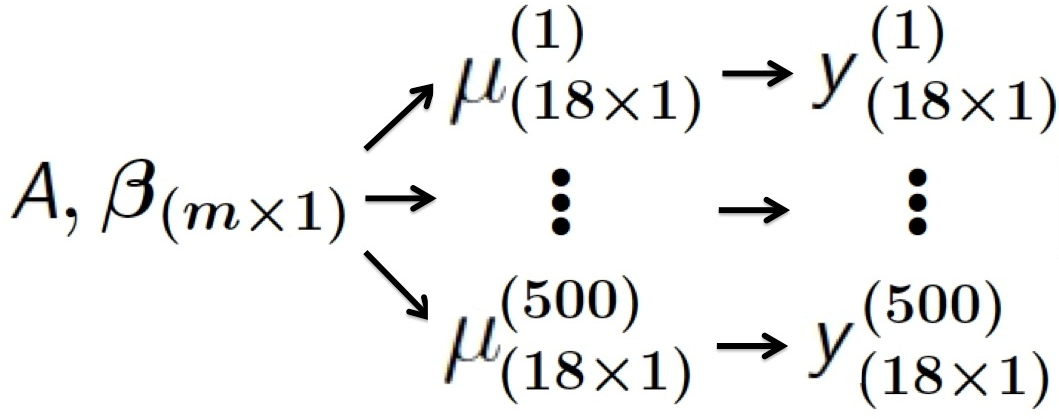
\includegraphics[width=6cm]{process.png}
\caption{Pseudo-data generating process}
\label{fig:pseudo}
\end{center}
\end{figure}

\subsection{Coverage Estimation Process}
Next, \code{coverage} fits the Normal-Normal model 500 times using the 500 pseudo-datasets in order to obtain 500$\times k$ interval estimates,  \{$(\hat{\mu}^{(i)}_{j, ~low}, ~\hat{\mu}^{(i)}_{j, ~upp}), ~j=1,\ldots, k,~ i=1, \ldots, 500$\}.  Here, we introduce both simple and Rao-Blackwellized unbiased coverage estimators but \code{coverage} displays only Rao-Blackwellized one.

\subsubsection{Simple Unbiased Coverage Estimates}
Let's define an indicator variable, $I^{(i)}_{j}$, which is 1 if the $j$-th group's interval estimate from the $i$-th pseudo-dataset includes $\mu^{(i)}_{j}$ and 0 otherwise. Then \code{coverage} estimates the coverage probability via the sample mean of these indicator variables for each group $j$, averaging over all the possible $\mu^{(i)}_{j}$ and $y^{(i)}_{j}$ for given $A$ and $\beta$. 
\begin{equation}
\bar{I}_{j}\equiv \frac{1}{N_{sim}}\sum_{i=1}^{N_{sim}}I^{(i)}_{j},~ j=1, 2, \ldots, k.
\end{equation}

This provides $k$ simple unbiased coverage estimates. For example, $\frac{1}{500}\sum_{i=1}^{500}I^{(i)}_{1}$ is the simple unbiased coverage estimate for the first group ($j=1$), accounting for possible randomness in $\mu^{(i)}_{1}$ and $y^{(i)}_{1}$, $i=1, \ldots, 500,$ given specific values of $A$ and $\beta$. 

Each indicator has the independent and identically distributed (\emph{iid}) Bernoulli($p_{cov, j}$) distribution, where $p_{cov, j}$ is the true coverage probability for the $j$-th group depending on specific values of $A$ and $\beta$.

Then, its unbiased variance estimator  for $Var(\bar{I}_{j})$ is simply the sample variance of indicators over the number of simulations.
\begin{equation}
\widehat{Var}(\bar{I}_{j})\equiv\frac{1}{N_{sim}(N_{sim}-1)}\sum_{i=1}^{N_{sim}}(I^{(i)}_{j}-\bar{I}_{j})^{2},~ j=1, 2, \ldots, k.
\end{equation}


\subsubsection{Rao-Blackwellized Unbiased Coverage Estimates}
Rao-Blackwellization improves accuracy of an unbiased estimator by taking more information (sufficient statistic) into account. Based on this idea, we use $E(I^{(i)}_{j}\vert y^{(i)}_{j}, A, \beta$), where $A$ and $\beta$ are given and $y^{(i)}_{j}$ is the sufficient statistic for the $j$-th group in the $i$-th pseudo-dataset. 
\begin{equation}\label{RB}
\bar{I}_{RB, j}\equiv \frac{1}{N_{sim}}\sum_{i=1}^{N_{sim}}E(I^{(i)}_{j}\vert y^{(i)}_{j}, A, \beta),~ j=1, 2, \ldots, k.
\end{equation}

The expectation in (\ref{RB}) is the same as Pr$(\hat{\mu}^{(i)}_{j, low}\le \mu^{(i)}_{j} \le\hat{\mu}^{(i)}_{j, upp}\vert y^{(i)}_{j}, A, \beta)$, where ($\hat{\mu}^{(i)}_{j, low}$, $\hat{\mu}^{(i)}_{j, upp}$) is the $j$-th group's interval estimate on the $i$-th dataset. We can calculate this probability  because we know the distribution of ($\mu^{(i)}_{j} \vert y^{(i)}_{j}, A, \beta$) in (\ref{normalpost}). Note that conditioning on $y^{(i)}_{j}$ is equivalent to conditioning on $\mathbf{y}^{(i)}_{(k\times1)}$ as long as $A$ and $\beta$ are known. 

For example, we estimate the first group's coverage probability (that depend on specific $A$ and $\beta$) by $\frac{1}{500}\sum_{i=1}^{500}E(I^{(i)}_{1}\vert y^{(i)}_{1}, A, \beta)$, which is also unbiased for $p_{cov, 1}$ but with smaller variance than the previous simple estimator, $\frac{1}{500}\sum_{i=1}^{500}I^{(i)}_{1}$.

Under the setting where one dataset ($\mathbf{y}^{(i)}_{(k\times1)}$) is simulated per one true parameter set ({\boldmath $\mu$}$^{(i)}_{(k\times1)})$, the unbiased variance estimator for Var($\bar{I}_{RB, j}$) follows.
\begin{equation}
\widehat{Var}(\bar{I}_{RB, j})\equiv\frac{1}{N_{sim}(N_{sim}-1)}\sum_{i=1}^{N_{sim}}\bigg(E(I^{(i)}_{j}\vert y^{(i)}_{j}, A, \beta)-\bar{I}_{RB, j}\bigg)^{2},~ j=1, 2, \ldots, k.
\end{equation}


\section[Examples]{Examples}
\subsection[Known Second-level Mean]{31 Hospitals: Known Second-level Mean}
\label{sec:ex:hosp}
In this example we adopt the perspective of a person living in the state of New York (NY) who has been suffering from severe coronary heart disease. If this person must receive coronary artery bypass graft (CABG) surgery soon, he or she might want to find the most reliable hospital for that.


For this purpose, data were gathered from 31 hospitals in NY composed of the number of deaths ($\textbf{z}_{(31\times1)}$) for a specified period after CABG surgeries and total number of patients ($\textbf{n}_{(31\times1)}$) receiving CABG surgeries in each hospital. For reference, caseloads ($n_{j}$) can be interpreted as exposures, not necessarily integers. These data can be loaded into R using the following code. Note that throughout this paper, the symbol `\code{R>}' represents a command prompt (not to be typed into \proglang{R}).

%For this purpose, data were gathered from 31 hospitals in NY composed of the number of deaths ($z$) for a specified period after CABG surgeries and total number of patients ($n$) receiving CABG surgeries in each hospital.  Suppose one knows that the state-level death rate per exposure of this surgery is 0.030 ($\lambda_{0}$). Using these data and the known second-level mean ($\lambda_{0}$), \pkg{Rgbp} provides point and interval estimates of the true death proportion for each hospital so that one can evaluate the hospital reliabilities. 


%These data, $\textbf{z}_{(31\times1)}$ and $\textbf{n}_{(31\times1)}$, can be loaded into R using the following code. Note that throughout this paper, the symbol `\code{R>}' represents a command prompt (not to be typed into \proglang{R}).

\begin{CodeChunk}
\begin{CodeInput}
R> z <- c(  3,  2,   5,  11,   9,  12,  12,   4,  10,  13,  14,   7,  12,
          11,  13,  22,  15,  11,  14,  11,  16,  14,   9,  15,  13,  35,
          26,  25,  20,  35,  27)
R> n <- c( 67, 68, 210, 256, 269, 274, 278, 295, 347, 349, 358, 396, 431,
         441, 477, 484, 494, 501, 505, 540, 563, 593, 602, 629, 636, 729,
         849, 914, 940, 1193, 1340)
\end{CodeInput}
\end{CodeChunk}
or
\begin{CodeChunk}
\begin{CodeInput}
R> data(hospitals)
R> z <- hospitals$d # variable name for the number of deaths is d in dataset
R> n <- hospitals$n
\end{CodeInput}
\end{CodeChunk}


In addition, suppose one knows that the state-level death rate per exposure of this surgery is 0.030 ($\lambda_{0}$). Using these data and the known second-level mean ($\lambda_{0}$), \pkg{Rgbp} provides point and interval estimates of the true death proportion for each hospital so that one can evaluate the hospital reliabilities. 


The independent Poisson distribution, \emph{i.e.},  $z_{j}\vert \lambda_{j}\stackrel{ind}{\sim} \textrm{Poisson}(n_{j}\lambda_{j})$, $j=1, \ldots, 31,$ would be an ideal choice to describe these data based on the Poisson approximation when $\lambda$ is small and $n$ is relatively big. 


Next, \code{gbp} will help us fit the Poisson hierarchical model with the Gamma conjugate prior distribution as the NY state-level population distribution of the true death rates ($\lambda_{j}$) whose mean is 0.030 ($\lambda_{0}=0.030$). For reference, the number of regression coefficients ($m$) is 0 because we do not need to estimate the prior mean via log-linear regression.
\begin{CodeChunk}
\begin{CodeInput}
R> p <- gbp(z, n, mean.PriorDist = 0.03, model = "poisson")
R> p
\end{CodeInput}
\begin{CodeOutput}
Summary for each unit (sorted by n):

         obs.mean    n prior.mean shrinkage low.intv post.mean upp.intv post.sd
1          0.0448   67       0.03     0.911   0.0199    0.0313   0.0454 0.00653
2          0.0294   68       0.03     0.910   0.0189    0.0299   0.0435 0.00631
3          0.0238  210       0.03     0.765   0.0185    0.0285   0.0407 0.00566
4          0.0430  256       0.03     0.728   0.0225    0.0335   0.0467 0.00619
5          0.0335  269       0.03     0.718   0.0208    0.0310   0.0432 0.00573
6          0.0438  274       0.03     0.714   0.0229    0.0339   0.0472 0.00621
7          0.0432  278       0.03     0.711   0.0228    0.0338   0.0469 0.00617
8          0.0136  295       0.03     0.699   0.0157    0.0250   0.0366 0.00534
9          0.0288  347       0.03     0.663   0.0200    0.0296   0.0410 0.00536
10         0.0372  349       0.03     0.662   0.0222    0.0325   0.0446 0.00571
11         0.0391  358       0.03     0.656   0.0228    0.0331   0.0454 0.00579
12         0.0177  396       0.03     0.633   0.0165    0.0255   0.0363 0.00506
13         0.0278  431       0.03     0.613   0.0200    0.0292   0.0400 0.00511
14         0.0249  441       0.03     0.608   0.0191    0.0280   0.0387 0.00502
15         0.0273  477       0.03     0.589   0.0199    0.0289   0.0394 0.00499
16         0.0455  484       0.03     0.585   0.0256    0.0364   0.0491 0.00601
17         0.0304  494       0.03     0.580   0.0211    0.0302   0.0409 0.00506
18         0.0220  501       0.03     0.577   0.0180    0.0266   0.0369 0.00483
19         0.0277  505       0.03     0.575   0.0202    0.0290   0.0395 0.00494
20         0.0204  540       0.03     0.559   0.0173    0.0258   0.0358 0.00474
21         0.0284  563       0.03     0.548   0.0206    0.0293   0.0395 0.00485
22         0.0236  593       0.03     0.535   0.0187    0.0270   0.0369 0.00466
23         0.0150  602       0.03     0.532   0.0147    0.0230   0.0329 0.00466
24         0.0238  629       0.03     0.521   0.0188    0.0271   0.0368 0.00460
25         0.0204  636       0.03     0.518   0.0173    0.0254   0.0351 0.00455
26         0.0480  729       0.03     0.484   0.0286    0.0393   0.0516 0.00587
27         0.0306  849       0.03     0.446   0.0223    0.0303   0.0397 0.00445
28         0.0274  914       0.03     0.428   0.0208    0.0285   0.0374 0.00423
29         0.0213  940       0.03     0.421   0.0176    0.0249   0.0335 0.00407
30         0.0293 1193       0.03     0.364   0.0223    0.0296   0.0379 0.00397
31         0.0201 1340       0.03     0.338   0.0170    0.0235   0.0310 0.00360
colMeans           517       0.03     0.600   0.0201    0.0293   0.0403 0.00517
\end{CodeOutput}
\end{CodeChunk}
For reference, we need to type `\code{R> print(p, sort = FALSE)}' instead of `\code{R> p}' in order to list hospitals by the order of data input in the above output. `\code{R> p}' automatically sorts the output by the increasing order of caseload ($n_{j}$), as shown above.


The output contains information about observed death ratios ($y_{j}$), caseloads ($n_{j}$), known prior mean ($\lambda_{0}$), shrinkage estimates ($\hat{B}_{j}$), lower bounds of interval estimates ($\hat{\lambda}_{j, low}$, 2.5\% percentiles of posterior distributions if 95\% confidence level is given), posterior means ($\hat{\lambda}_{j}=E(\lambda_{j}\vert \textbf{y})$), upper bounds  of interval estimates ($\hat{\lambda}_{j, upp}$, 97.5\% percentiles of posterior distributions), and standard deviations of posterior distributions ($sd(\lambda_{j}\vert \textbf{y})$).


As we can see in (\ref{gammapost}), the posterior mean, $(1-B_{j})y_{j} + B_{j}\lambda_{0}$, is a convex combination of the sample mean and prior mean ($\lambda_{0}=0.030$) with the shrinkage factor, $B_{j}\equiv r / (r + n_{j})$, determining the weight. This makes intuitive sense because $r$ and $n_{j}$ can be interpreted as the degree (sample sizes) of prior and observed information respectively. If the second level has more information than the first level, \emph{i.e.} ensemble sample size $r$ exceeds individual sample size $n_{j}$, then the estimator will shrink towards the prior mean more than 50\%. This is clear because, as caseload increases, shrinkage decreases, depending less on the second-level information.


A function \code{summary} shows selective information on hospitals and more detailed estimation results, as below. To be specific, it displays some hospitals (not all as above) with minimum, median, and maximum caseloads ($n_{j}$). On top of that, more specific estimation results, such as the posterior mode and standard deviation of $\alpha\equiv\log(1/r)$, follow. When we do not know the prior mean in advance, unlike this hospital problem, \code{gbp} always fits the natural link, \emph{i.e.} a linear regression for the Normal model, a log-linear regression for the Poisson model, and a logistic regression for the Binomial model.
\begin{CodeChunk}
\begin{CodeInput}
R> summary(p)
\end{CodeInput}
\begin{CodeOutput}
Main summary:

                    obs.mean    n prior.mean shrinkage low.intv post.mean
Unit with min(n)      0.0448   67       0.03     0.911   0.0199    0.0313   
Unit with median(n)   0.0455  484       0.03     0.585   0.0256    0.0364   
Unit with max(n)      0.0201 1340       0.03     0.338   0.0170    0.0235   
Overall Mean                  517       0.03     0.600   0.0201    0.0293   

                    upp.intv  post.sd
                      0.0454  0.00653
                      0.0491  0.00601
                      0.0310  0.00360
                      0.0403  0.00517

Second-level Variance Component Estimation Summary:
alpha = log(A) for Gaussian or alpha = log(1/r) for Binomial and Poisson data:

  post.mode.alpha post.sd.alpha post.mode.r
1           -6.53         0.576         684
\end{CodeOutput}
\end{CodeChunk}
The output of \code{summary} also provides $\hat{r}=\textrm{exp}(6.53)=684$, which is an indicator of how valuable and informative the hypothetical second-level hierarchy is. It means that observed sample means of hospitals whose caseloads are less than 684 will shrink toward the prior mean (0.030) more than 50\%. For example, the shrinkage estimate of the first hospital ($\hat{B}_{1}= 0.911$) was calculated by 684 / (684 + 67), where 67 is its caseload ($n_{1}$), and its posterior mean is $(1-0.911)*0.0448 + 0.911 * 0.030=0.0313$. As for this hospital, using more information from the prior distribution is an appropriate choice because the observed amount of information (67) is far less than the amount of state-level information (684).


To obtain a graphical summary the function \code{plot} can be used, as seen in Figure \ref{fig:hospshr}.

\begin{CodeChunk}
\begin{CodeInput}
R> plot(p)
\end{CodeInput}
\end{CodeChunk}
\begin{figure}[h]
\begin{center}
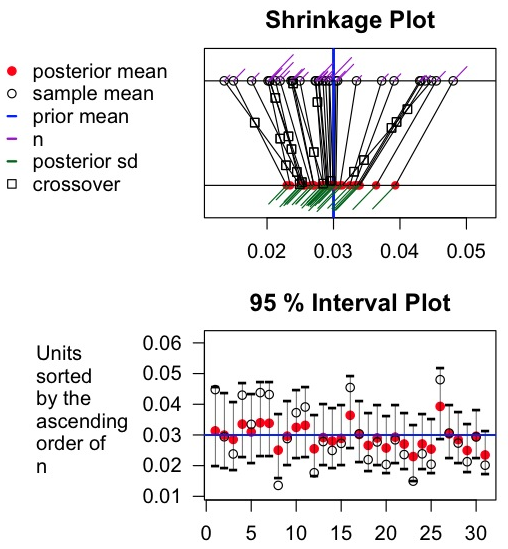
\includegraphics[width = 6in]{hospital1.png}
\caption{Shrinkage plot and 95\% interval plot for 31 hospitals}
\label{fig:hospshr}
\end{center}
\end{figure}

In Figure \ref{fig:hospshr} the regression towards the mean (RTTM) is obvious in the first graph; the observed sample means, empty dots on the upper horizontal line, are shrinking towards the known second-level mean (a blue vertical line at 0.030) to the different extents. Note that some hospitals' ranks have changed by shrinking much harder towards 0.030 than others. For example, the empty square symbol at the crossing point of the two left-most lines (8th and 23rd hospitals on the list above) indicates that seemingly the safest hospital among 31 hospitals in terms of the observed death ratio is not actually safer than seemingly the second safest hospital. 


Intuitively, switching ranks for these two hospitals makes sense. To be specific, their observed death rates ($y_{j}$, $j=8, 23$) are 0.0136 and 0.0150 and caseloads ($n_{j}$, $j=8, 23$) are 295 and 602 each. Considering solely the observed death rates may lead to an unfair comparison because the latter hospital handled twice the caseload. \pkg{Rgbp} accounts for this caseload difference, making the true death rate estimate for the former hospital shrink toward the state-level mean ($\lambda_{0}$=0.030) much harder than that for the latter hospital. This is what happened to the two left-most hospitals in the first plot.


But the point estimates are not enough to evaluate hospital reliabilities because one hospital may have a lower point estimate but  bigger uncertainty (variance) than the other. In the second plot of Figure \ref{fig:hospshr}, the estimated 95\% intervals are displayed. We see that each posterior mean (red dot) is between the sample mean (empty dot) and the second-level mean (a blue horizontal line). For reference, we could plot this 95\% interval plot by the order of data input via \code{plot(p, sort = FALSE)}.

This 95\% interval plot reveals that the 31st hospital has the lowest upper bound of 95\% interval estimate, although its point estimate ($\hat{\lambda}_{31}=0.0235$) is slightly bigger than that of the 23rd hospital ($\hat{\lambda}_{23}=0.0230$). Let's see the details of these two hospitals. The observed death rates for these two hopitals ($y_{j}, j=23, 31$) are 0.0150 and 0.0201 and the caseloads ($n_{j}, j =23, 31$) are 602 and 1340 each. The 31st hospital has twice the caseload, which leads to borrowing less information from the NY state-level hierarchy (or shrinking less toward the state-level mean, 0.030) with smaller variance.

%and What happened is that Since the 23rd hospital has the lowest upper bound for the true death rate, not to mention the lowest point estimate. Also it reveals that the 31st hospital may be the second safest because its upper bound of 95\% interval estimate for the true death rate is lower than the 8th hospital's one.


%From the output provided by \code{gbp} it can be seen that a reasonable choice of a hospital for the patient is hospital 23. Although hospital 8 has a smaller observed mean the fact that hospital 23 has a much higher caseload means that we borrow relatively less information from other hospitals. The result being that the upper bound of the $95\%$ interval is smaller.

%provides one more point, which we could not have noticed. Let's look at the 8th and the 31st hospitals on the graph (or on the outcome for numeric reference). The point estimate of the true death rate per exposure of the 31st hospital is higher than the one of the 8th. But, the upper bound of interval estimate of this 31st hospital is lower than that of the 8th. This interval plot makes the 31st hospital emerge as one of your candidates.


% Also it reveals that the 23rd hospital, whose estimated true rate was the smallest, has also the smallest upper bound. If you are a risk-adverse, this hospital will attract you most strongly. And if you already chose this 23rd hospital compared to the 8th from the shrinkage plot, your decision might become stronger at this point, excluding the 8th hospital with more certainty. 

Based on the point and interval estimates, the 31st hospital seems the most reliable one among all the candidates. But when fitting a model it is always a good idea to question how reliable the estimation procedure is. For example, does our procedure generate interval estimates that have good repeated sampling properties? To answer this question the \code{coverage} function generates pseudo-datasets assuming the estimated $r~(=683.53)$ is a true value. For reference, We also could try any other value of $r$, for example $r=600$, by adding another argument, \code{A.or.r = 600}, into the code below; \code{R> pcv <- coverage(p, A.or.r = 600, nsim = 1000)}.



Also, \code{gbp} provides interval estimates with different confidence levels, for example 90\%. For this, we need to go back to the code for fitting the model, adding another argument, \code{Alpha = 0.9}; \code{R> p <- gbp(z, n, Alpha = 0.9, mean.PriorDist = 0.03, model = "poisson")}.  Then, the code below will evaluate whether interval estimates achieve the 90\% confidence level.

\begin{CodeChunk}
\begin{CodeInput}
R> pcv <- coverage(p, nsim = 1000)
\end{CodeInput}
\end{CodeChunk}
\begin{figure}[h] 
\begin{center}
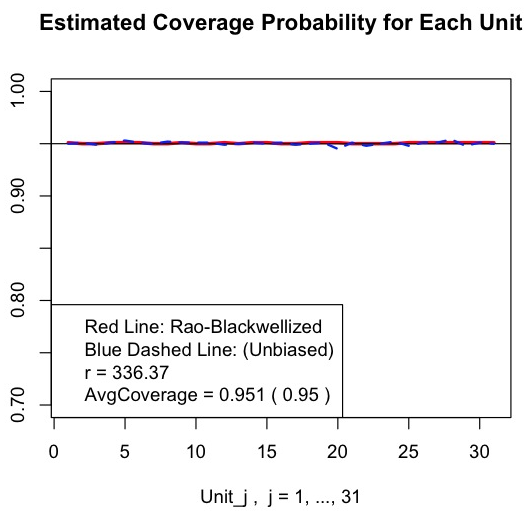
\includegraphics[width = 3.5in]{hospital2.png}
\caption{Coverage plot via frequency method checking for 31 hospitals}
\label{fig:hospitalcoverage}
\end{center}
\end{figure}

In Figure \ref{fig:hospitalcoverage}, the black horizontal line at 0.95 represents the nominal confidence level and the smooth red curve connects Rao-Blackwellized (RB) unbiased coverage estimates for 31 hospitals.



The overall RB unbiased coverage estimate across all the hospitals is 0.954. And none of RB unbiased coverage estimates for 31 hospitals are less than 0.95 regardless of their caseloads ($n_{j}$). This result shows that the interval estimates for this particular dataset accurately achieves 95\% confidence under repeated sampling. Note that these estimates depend on the given true value of $r$, the known prior mean, and the assumption that the model is true.

The following code provides 31 RB unbiased coverage estimates for each hospital.
\begin{CodeChunk}
\begin{CodeInput}
R> pcv$coverageRB
\end{CodeInput}
\begin{CodeOutput}
 [1] 0.956 0.956 0.956 0.955 0.955 0.955 0.955 0.955 0.955 0.955 0.955 0.954 
[13] 0.955 0.954 0.954 0.954 0.954 0.954 0.955 0.954 0.954 0.953 0.953 0.953
[25] 0.954 0.954 0.954 0.953 0.953 0.953 0.952
\end{CodeOutput}
\end{CodeChunk}

And the code below calculates 31 simple unbiased coverage estimates for each hospital.
\begin{CodeChunk}
\begin{CodeInput}
R> pcv$coverageS
\end{CodeInput}
\begin{CodeOutput}
 [1] 0.947 0.952 0.963 0.961 0.957 0.957 0.959 0.952 0.957 0.957 0.941 0.958 
[13] 0.954 0.962 0.935 0.940 0.955 0.952 0.951 0.941 0.955 0.952 0.954 0.946 
[25] 0.942 0.952 0.958 0.945 0.938 0.958 0.948
\end{CodeOutput}
\end{CodeChunk}

The function \code{coverage} also calculates the standard errors for each hospital's RB unbiased coverage estimate defined as the square root of $S^{2}_{RB, j}/N_{sim}$, where $S^{2}_{RB, j}$ is the sample variance of 1,000 RB unbiased coverage estimates for the $j$-th hospital. The following code provides 31 standard errors.
\begin{CodeChunk}
\begin{CodeInput}
R> pcv$se.coverageRB
\end{CodeInput}
\begin{CodeOutput}
 [1] 0.0017 0.0017 0.0014 0.0014 0.0014 0.0014 0.0014 0.0014 0.0013 0.0013 0.0013 
[12] 0.0013 0.0012 0.0012 0.0012 0.0012 0.0011 0.0012 0.0011 0.0011 0.0011 0.0011
[23] 0.0010 0.0011 0.0010 0.0010 0.0009 0.0009 0.0009 0.0007 0.0007
\end{CodeOutput}
\end{CodeChunk}
Similarly, 31 standard errors for each simple unbiased coverage estimate are
\begin{CodeChunk}
\begin{CodeInput}
R> pcv$se.coverageS
\end{CodeInput}
\begin{CodeOutput}
 [1] 0.0071 0.0068 0.0060 0.0061 0.0064 0.0064 0.0063 0.0068 0.0064 0.0064 0.0075 
[12] 0.0063 0.0066 0.0060 0.0078 0.0075 0.0066 0.0068 0.0068 0.0075 0.0066 0.0068 
[23] 0.0066 0.0072 0.0074 0.0068 0.0063 0.0072 0.0076 0.0063 0.0070
\end{CodeOutput}
\end{CodeChunk}

Taking the first hospital as an example, the variance estimate of RB unbiased coverage estimate is about 17 times smaller than that of simple one. It means that 1,000 RB unbiased coverage estimates are as precise as 17,000 simple unbiased coverage estimates in terms of estimating true coverage probability for the first hospital.

For reference, two $31 \times 1,000$ matrices \code{raw.resultRB} and \code{raw.resultS}, each row of which is about each hospital, in \code{pcv} contain all the individual estimates.
% For reference, it took 10 seconds for MacBook Pro with a 2.3 GHz dual-core Intel i5 CPU to run 10,000 simulations.


%These numbers are encouraging, but achieving at least 95\% coverage at %one specific true value does not mean that our model has good repeated %sampling property. We need to check whether coverage probabilities are %at least 0.95 when the true parameter value ($r$) varies.

%\begin{CodeChunk}
%\begin{CodeInput}
%R> shr <- seq(0.01, 0.99, length.out = 20)
%R> r.trial <- mean(n) * shr / (1 - shr)
%R> cov.save <- sapply (1 : length(r.trial), function(i){
%R>               coverage(p, A.or.r = r.trial[i], mean.PriorDist = 0.02, 
%R>                        nsim = 500)$average.coverageRB
%R>             })
%\end{CodeInput}
%\end{CodeChunk}
%\begin{figure}[h]
%\begin{center}
%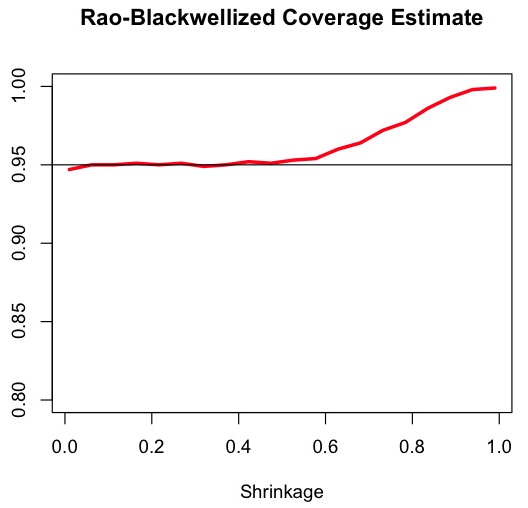
\includegraphics[width = 5.5cm]{hospital3.png}
%\end{center}
%\end{figure}

%We plotted \code{cov.save} on \code{shr}, connecting dots (coverage %probabilities). This plot shows that the estimated shrinkages are at least %0.947 (under 95\% only at one shrinkage value, 0.01) on the tried range %of true shrinkage values, slightly deviating from the definition of 95\% %confidence interval. Note that our model is approximating the true %distribution of shrinkage by ADM (see 4.2). 

%The reason we tried true shrinkage values between 0.01 and 0.99 is that no shriankge ($\equiv r / (r + n_{j})=0)$, corresponding to $r=0$, makes the scale of the distribution go to $\infty$ (see (5)), and full shrinkage ($B_{j}=1$) makes $r$ goes to $\infty$, not appropriate for an argument.

\cite{1995} also investigated a similar ranking problem in hierarchical modeling, taking shrinkage into account.


\subsection[Unknown Second-level Mean and No Covariate]{8 Schools: Unknown Second-level Mean and No Covariate} \label{sec:ex:8schools}

The Education Testing Service (ETS) conducted randomized experiments in eight separate schools (group) to test whether students (unit) SAT scores are effected by coaching. The dataset contains the estimated coaching effects on SAT scores ($y_{j}, j=1, \ldots, 8$) and standard errors ($se_{j}, j=1, \ldots, 8$) of the eight schools \citep{1981}.
\begin{CodeChunk}
\begin{CodeInput}
R> y  <- c(12, -3, 28,  7,  1,  8, 18, -1)
R> se <- c(18, 16, 15, 11, 11, 10, 10,  9)
\end{CodeInput}
\end{CodeChunk}
or
\begin{CodeChunk}
\begin{CodeInput}
R> data(schools)
R> y  <- schools$y
R> se <- schools$se
\end{CodeInput}
\end{CodeChunk}



Due to the nature of the test each school's coaching effect has an approximately Normal sampling distribution with known sampling variance, \emph{i.e.}, standard error of each school is assumed to be known. At the second hierarchy, the mean for each school is assumed to be drawn from a common Normal distribution and hence, we can use the Gaussian component of \code{gbp} to fit this Normal-Normal hierarchical model.


\begin{CodeChunk}
\begin{CodeInput}
R> g <- gbp(y, se, model = "gaussian")
R> g
\end{CodeInput}
\begin{CodeOutput}
Summary for each unit (sorted by se):

         obs.mean   se prior.mean shrinkage low.intv post.mean upp.intv post.sd
5           -1.00  9.0      8.168     0.408  -13.297     2.737   16.692   7.634
2            8.00 10.0      8.168     0.459   -7.255     8.077   23.361   7.810
7           18.00 10.0      8.168     0.459   -1.289    13.484   30.821   8.176
4            7.00 11.0      8.168     0.507   -8.780     7.592   23.602   8.257
6            1.00 11.0      8.168     0.507  -13.027     4.633   20.131   8.441
1           28.00 15.0      8.168     0.657   -2.315    14.979   38.763  10.560
3           -3.00 16.0      8.168     0.685  -17.130     4.650   22.477  10.096
8           12.00 18.0      8.168     0.734  -10.208     9.189   29.939  10.227
colMeans          12.5      8.168     0.552   -9.163     8.168   25.723   8.900
\end{CodeOutput}
\end{CodeChunk}
This output from \code{gbp} summarizes the results. In this Normal-Normal hierarchical model the amount of shrinkage for each unit is governed by the shrinkage factor, $B_j = V_j/(V_j + A)$. As such, schools whose variation within the school ($V_{j}$) is less than the between variation ($A$) schools will shrink greater than $50\%$. The results provided by \code{gpb} suggests that there is little evidence that the training provided much added benefit due to the fact that every school's $95\%$ posterior interval contains 0. 

\begin{CodeChunk}
\begin{CodeInput}
R> plot(g)
\end{CodeInput}
\end{CodeChunk}

\begin{figure}[h] 
\begin{center}
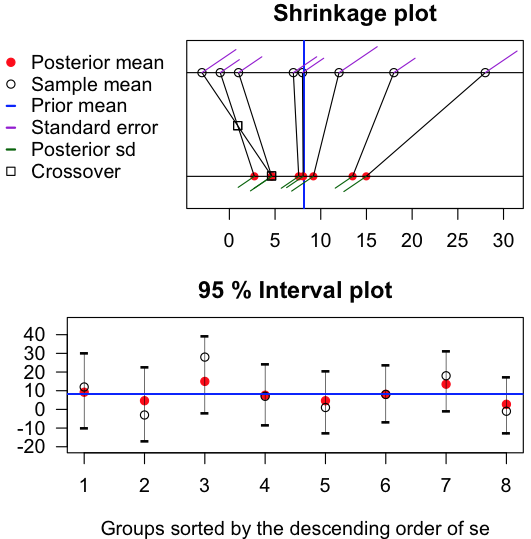
\includegraphics[width = 6in]{school1.png}
\caption{Shrinkage plot and 95\% interval plot for 8 schools}
\label{fig:8schoolsplot}
\end{center}
\end{figure}

\pkg{Rgbp} also provides functionality to plot the results of the analysis as seen in Figure \ref{fig:8schoolsplot}. Plotting the results provides a visual aid to understanding but is only largely beneficial when the number of groups $(k)$ is small. In the case where the number of groups is large \pkg{Rgbp} provides a summary feature:

\begin{CodeChunk}
\begin{CodeInput}
R> summary(g)
\end{CodeInput}
\begin{CodeOutput}
Main summary:

                      obs.mean   se prior.mean shrinkage low.intv post.mean
Unit with min(se)        -1.00  9.0       8.17     0.408   -13.30      2.74     
Unit with median(se)1     1.00 11.0       8.17     0.507   -13.03      4.63     
Unit with median(se)2     7.00 11.0       8.17     0.507    -8.78      7.59     
Unit with max(se)        12.00 18.0       8.17     0.734   -10.21      9.19     
Overall Mean                   12.5       8.17     0.552    -9.16      8.17     

                      upp.intv post.sd
                          16.7    7.63
                          20.1    8.44
                          23.6    8.26
                          29.9   10.23
                          25.7    8.90

Second-level Variance Component Estimation Summary:
alpha = log(A) for Gaussian or alpha =  log(1/r) for Binomial and Poisson data:

  post.mode.alpha post.sd.alpha post.mode.A
1            4.77          1.14         118


Regression Summary:

      estimate   se z.val p.val
beta0    8.168 5.73 1.425 0.154
\end{CodeOutput}
\end{CodeChunk}


The method check, assuming the model is correct, generates new pseudo-data from our assumed model. It starts by fixing the hyper-parameter values at their estimates ($\hat{A}$ and $\hat{\beta}_0$ in this example). We then simulate ``true'' $\theta_j$ for each group $j$ and re-fit the model 1,000 times to estimate the coverage probabilities of our procedure.  

\begin{CodeChunk}
\begin{CodeInput}
R> gcv <- coverage(g, nsim = 1000)
\end{CodeInput}
\end{CodeChunk}
\begin{figure}[h] 
\begin{center}
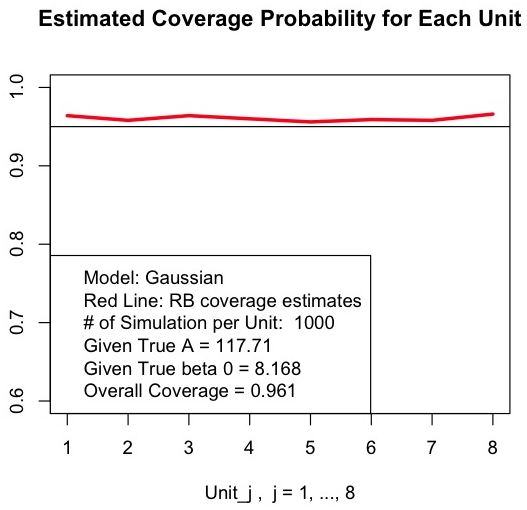
\includegraphics[width = 3.5in]{school2.png}
\caption{Coverage plot via frequency method checking for 8 schools}
\label{fig:schoolcoverage}
\end{center}
\end{figure}

As seen in Figure \ref{fig:schoolcoverage} the desired $95\%$ confidence (black horizontal line at 0.95) is achieved (actually, exceeded) for each school in this example. Note that all the coverage estimates depend on the chosen true values of $A$ and $\beta_{0}$, and the assumption that the model is valid.


In addition, Rao-Blackwellized (RB) unbiased coverage estimate and its standard error for each school can be gotten with the command below.
\begin{CodeChunk}
\begin{CodeInput}
R> gcv$coverageRB
\end{CodeInput}
\begin{CodeOutput}
 [1] 0.966 0.959 0.967 0.960 0.959 0.962 0.960 0.966
\end{CodeOutput}
\end{CodeChunk}
\begin{CodeChunk}
\begin{CodeInput}
R> gcv$se.coverageRB
\end{CodeInput}
\begin{CodeOutput}
 [1] 0.0013 0.0012 0.0013 0.0013 0.0011 0.0011 0.0010 0.0017
\end{CodeOutput}
\end{CodeChunk}

All the individual RB coverage estimates are saved in the $8\times1,000$ matrix, \code{gcv$raw.resultRB}, each row of which is about each school.


% For reference, it took 188 seconds for 10,000 simulations  on one of authors' MacBook Pro with a 2.3 GHz dual-core Intel i5 CPU. In MCMC, the exact simulation would be too time-consuming. One could compare curve in Figure \ref{fig:schoolcoverage} with a curve from MCMC.

%\begin{CodeChunk}
%\begin{CodeInput}
%R> shr <- seq(0.01, 0.99, length.out = 20)
%R> A.trial <- mean(n) * (1 - shr) / shr
%R> cov.save <- sapply (1 : length(A.trial), function(i){
%R>               coverage(g, A.or.r = A.trial[i], reg.coef = 8.168, 
%R>                        nsim = 500)$average.coverageRB
%R>             })
%\end{CodeInput}
%\end{CodeChunk}
%\begin{figure}[h]
%\begin{center}
%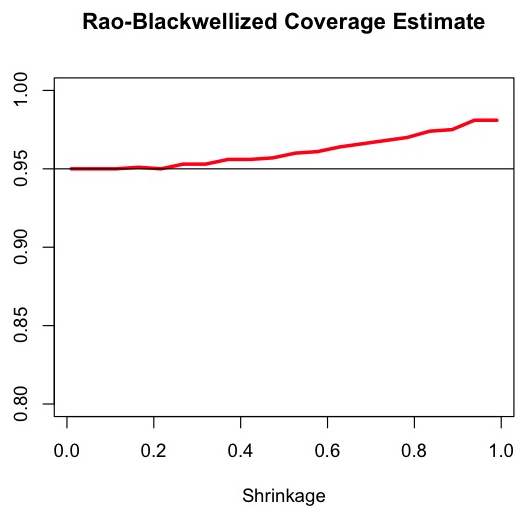
\includegraphics[width = 5.5cm]{school3.png}
%\end{center}
%\end{figure}


\subsection[Unknown Second-level Mean and One Covariate]{18 Baseball Players: Unknown Second-level Mean and One Covariate}
%The New York Times published on 26 April 1970 covered 18 baseball players' batting averages through their first official 45 at-bats of the 1970 season. And then we became interested in their batting averages over the remaining season. 

The following dataset from the New York Times published on 26 April 1970 contains information on the batting averages and positions (outfielder=1,otherwise=0) of 18 major league baseball players through their first 45 official at-bats of the 1970 season \citep{1975}.

\begin{CodeChunk}
\begin{CodeInput}
R> z <- c(18, 17, 16, 15, 14, 14, 13, 12, 11, 11, 10, 10, 10, 10, 10,  9,  8,  7)
R> n <- c(45, 45, 45, 45, 45, 45, 45, 45, 45, 45, 45, 45, 45, 45, 45, 45, 45, 45)
R> x <- c( 1,  1,  1,  1,  1,  0,  0,  0,  0,  1,  0,  0,  0,  1,  1,  0,  0,  0) 
\end{CodeInput}
\end{CodeChunk}
or
\begin{CodeChunk}
\begin{CodeInput}
R> data(baseball)
R> z <- baseball$Hits
R> n <- baseball$At.Bats
R> x <- ifelse(baseball$Position == "fielder", 1, 0)
\end{CodeInput}
\end{CodeChunk}
%$
Conditioning on the true batting average for each player we assume that the at-bats are independent and therefore, $z_{j}\vert p_{j}\stackrel{ind}{\sim} \textrm{Binomial}(45, p_{j}), ~j=1, \ldots, 18$. Our goal is to obtain point and interval estimates of the true batting average, $p_{j}$, for each player, whilst considering the additional information on whether the player is an outfielder or not. \code{gbp} provides a way to incorporate such covariate information seamlessly into the second-level hierarchy such that information is shared and regression towards the mean (RTTM) occurs within outfielders and non-outfielders separately. %For reference, we can also assume the Normal distribution using $y_{j}=z_{j} / n_{j}$ and $V_{j}=\bar{y}(1-\bar{y})/n$, where $\bar{y}=\sum_{j} z_{j} / \sum_{j} n_{j}$, $j=1,\ldots, 18$. 


\begin{CodeChunk}
\begin{CodeInput}
R> b <- gbp(z, n, x, model = "binomial")
R> b
\end{CodeInput}
\begin{CodeOutput}
Summary for each unit (sorted by n):

         obs.mean  n   X1 prior.mean shrinkage low.intv post.mean upp.intv post.sd
1           0.400 45 1.00      0.310     0.715    0.248     0.335    0.429  0.0462
2           0.378 45 1.00      0.310     0.715    0.244     0.329    0.420  0.0448
3           0.356 45 1.00      0.310     0.715    0.240     0.323    0.411  0.0437
4           0.333 45 1.00      0.310     0.715    0.236     0.316    0.403  0.0429
5           0.311 45 1.00      0.310     0.715    0.230     0.310    0.396  0.0424
6           0.311 45 0.00      0.233     0.715    0.179     0.256    0.341  0.0415
7           0.289 45 0.00      0.233     0.715    0.175     0.249    0.331  0.0400
8           0.267 45 0.00      0.233     0.715    0.171     0.243    0.323  0.0388
9           0.244 45 0.00      0.233     0.715    0.166     0.237    0.315  0.0380
10          0.244 45 1.00      0.310     0.715    0.210     0.291    0.379  0.0432
11          0.222 45 0.00      0.233     0.715    0.161     0.230    0.308  0.0377
12          0.222 45 0.00      0.233     0.715    0.161     0.230    0.308  0.0377
13          0.222 45 0.00      0.233     0.715    0.161     0.230    0.308  0.0377
14          0.222 45 1.00      0.310     0.715    0.202     0.285    0.375  0.0441
15          0.222 45 1.00      0.310     0.715    0.202     0.285    0.375  0.0441
16          0.200 45 0.00      0.233     0.715    0.155     0.224    0.302  0.0377
17          0.178 45 0.00      0.233     0.715    0.148     0.218    0.297  0.0381
18          0.156 45 0.00      0.233     0.715    0.140     0.211    0.292  0.0389
colMeans          45 0.44      0.267     0.715    0.191     0.267    0.351  0.0410
\end{CodeOutput}
\end{CodeChunk}
% Our model reflects on the additional information, \emph{i.e.}, indicator covariate (1 for outfielder and 0 for other positions), estimating two different prior means, 0.310 and 0.233. Also
Note that the shrinkage estimates are the same for all players due to the fact that they are determined solely by the relative amount of information between the first-level and the second-level hierarchies, ($\hat{B}_{j}\equiv \hat{r} / (\hat{r}+45)$ = $113 / (113+45)$ = 0.715). 

%Note that the posterior standard deviation tends to be bigger among outfielders than among others. Let's see its formula in (9). We can notice that the estimated posterior mean is a critical factor that makes posterior variances different from each player because every player has the same at-bats ($n_{j}$) and $r$. As the posterior mean gets closer to 0.5, the posterior variance gets bigger and has the biggest value when the posterior mean is 0.5. Intuitively, it makes sense. If a true batting average is 0.1, we can easily expect less hits. But if it is 0.5, we are less certain whether an at-bat would be more likely a hit or not, like a coin tossing. Our model is automatically reflecting on such uncertainty.

%In problems where a covariate is present \code{gbp} provides a regression summary (in this example logistic regression)
\begin{CodeChunk}
\begin{CodeInput}
R> summary(b)
\end{CodeInput}
\begin{CodeOutput}
Main summary:

                            obs.mean  n    X1 prior.mean shrinkage low.intv 
Unit with min(obs.mean)        0.156 45 0.000      0.233     0.715    0.140     
Unit with median(obs.mean)1    0.244 45 0.000      0.233     0.715    0.166     
Unit with median(obs.mean)2    0.244 45 1.000      0.310     0.715    0.210     
Unit with max(obs.mean)        0.400 45 1.000      0.310     0.715    0.248     
Overall Mean                         45 0.444      0.267     0.715    0.191     


                            post.mean upp.intv post.sd
                                0.211    0.292  0.0389
                                0.237    0.315  0.0380
                                0.291    0.379  0.0432
                                0.335    0.429  0.0462
                                0.267    0.351  0.0410

Second-level Variance Component Estimation Summary:
alpha = log(A) for Gaussian or alpha =  log(1/r) for Binomial and Poisson data:

  post.mode.alpha post.sd.alpha post.mode.r
1           -4.73         0.957         113


Regression Summary:

      estimate    se  z.val p.val
beta0   -1.194 0.131 -9.129 0.000
beta1    0.389 0.187  2.074 0.038
\end{CodeOutput}
\end{CodeChunk}

From the output summary we see that the two prior means distinguishing outfielders from other positions are statistically significantly different (p-value = 0.038). Also, the positive sign of $\hat{\beta}_{1}$ indicates that the population mean batting average for all outfielders tends to be higher than that for those in the other positions (estimated odds ratio = exp(0.389)=1.48).

\begin{CodeChunk}
\begin{CodeInput}
R> plot(b)
\end{CodeInput}
\end{CodeChunk}
\begin{figure}[h]
\begin{center}
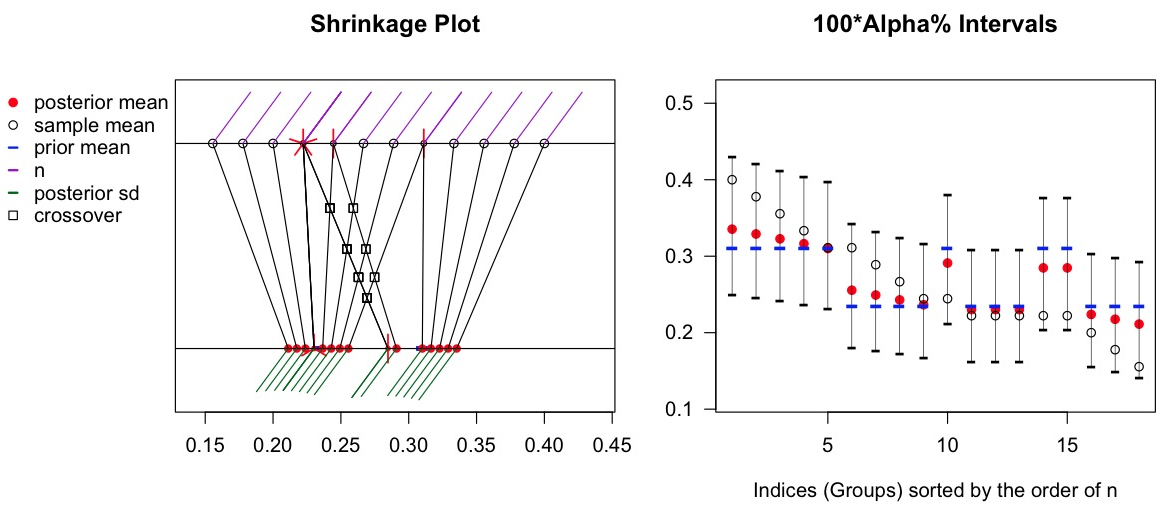
\includegraphics[width = 6in]{baseball1.png}
\caption{Shrinkage plot and 95\% interval plot for 18 baseball players}
\label{fig:baseball}
\end{center}
\end{figure}

It is evident in the shrinkage plot in Figure \ref{fig:baseball} that shrinkage occurs from the sample means (empty dots) on the upper horizontal line towards the two prior means, 0.233 and 0.310. For reference, the red line symbols on dots are for when two or more points have the same mean and are plotted over each other. For example, five players (from the 11th player to the 15th) have the same sample mean (0.222) and at this point on the upper horizontal line, there are short red lines toward five directions.

%For reference, the observed sample mean among outfielders is 0.308 and that among other positions is 0.231. But why are the estimated two prior means from this Binomial model 0.310 and 0.233 each? This can be attributed to the logistic regression which estimates prior mean by a non-linear logit function of $x'\beta$, causing a small bias (see 3.3). The Normal model can avoid this small bias because it uses a linear regression to estimate these prior means.


The 95\% interval plot shows the range of true batting average for each player, which clarifies the regression toward the mean (RTTM) within two groups. The 10th, 14th, and 15th players, for example, are outfielders but their observed batting averages are far lower than the first five outfielders. RTTM suggests that in the long run their batting averages will shrink toward the expected prior means as outfielders (blue horizontal lines).


As in the previous examples in Sections \ref{sec:ex:hosp} and \ref{sec:ex:8schools} to check the level of trust in these interval estimates a method check can be undertaken by assuming the estimates, $\hat{r}$ (=112.95) and $\hat{\beta}~(=(-1.194, ~0.389)^{T})$, are true values. 

\begin{CodeChunk}
\begin{CodeInput}
R> bcv <- coverage(b, nsim = 1000) 
\end{CodeInput}
\end{CodeChunk}
\begin{figure}[h]
\begin{center}
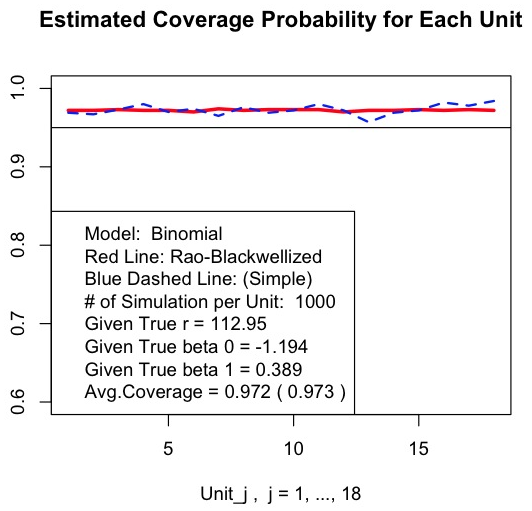
\includegraphics[width = 3.5in]{baseball2.png}
\caption{Coverage plot via frequency method checking for 18 players}
\label{fig:baseball2}
\end{center}
\end{figure}

For reference, to do the method check at different true values additional arguments can be specified in the coverage function. For example, if we want to try different true values, either 100 for $r$ or (-1, 0.2) for $(\beta_{0}, \beta_{1})$, the additional arguments are \code{A.or.r = 100} and \code{reg.coef = c(-1, 0.2)}; \code{coverage(b, A.or.r = 100, reg.coef = c(-1, 0.2), nsim = 1000)} instead of the above code.


Finally, in Figure \ref{fig:baseball2}, we see that the overall Rao-Blackwellized unbiased coverage estimate is 0.972 (across all the players), conservatively satisfying the definition of the 95\% confidence interval. Note that each coverage estimate depends on given true values of $r$ and $\beta_{(2\times1)}$, and the assumption that the model is valid.


The Rao-Blackwellized unbiased coverage estimates and their standard errors for each player follow.
\begin{CodeChunk}
\begin{CodeInput}
R> bcv$coverageRB
\end{CodeInput}
%$
\begin{CodeOutput}
 [1] 0.972 0.973 0.973 0.973 0.972 0.972 0.972 0.972 0.973 0.972 0.973 0.972 
[13] 0.973 0.973 0.971 0.973 0.971 0.973
\end{CodeOutput}
\end{CodeChunk}
\begin{CodeChunk}
\begin{CodeInput}
R> bcv$se.coverageRB
\end{CodeInput}
\begin{CodeOutput}
 [1] 0.0015 0.0011 0.0012 0.0011 0.0015 0.0012 0.0012 0.0010 0.0011 0.0012 
[11] 0.0010 0.0012 0.0010 0.0011 0.0013 0.0011 0.0013 0.0010
\end{CodeOutput}
\end{CodeChunk}

%$

All the simulation results are saved in the $18\times1,000$ matrix, \code{bcv$raw.resultRB}, each row of which is for each player.

%$


%Finally,  we see that Rao-Blackwellized unbiased estimate for the first player is about 26 times more accurate than simple one. It is based on the ratio of the sample variances of individual estimates from two approaches.
%\begin{CodeChunk}
%\begin{CodeInput}
%R> var(bcv$raw.resultS[1, ]) / var(bcv$raw.resultRB[1, ])
%\end{CodeInput}
%\begin{CodeOutput}
% [1] 25.64346
%\end{CodeOutput}
%\end{CodeChunk}
% As for the running time, it took 243 seconds for MacBook Pro equipped with a 2.3 GHz dual-core Interl i5 CPU to execute 10,000 simulations.


%However, achieving at least 95\% coverage at specific true values of $r$ and $\beta$ does not mean that our model has good repeated sampling property. So, as we did in previous examples, we will see whether coverage probabilities are at least 0.95 when the true shrinkage value ($B(r)$) varies, fixing $\beta$ at estimated values. Note that, if we want to check a coverage probability under the different parameter values, $r$ and $\beta$, for example 150 for $r$ and $(-1, 0.5)^{T}$ for $\beta$, the appropriate code is \code{R> coverage(b, A.or.r = 150, reg.coef = c(-1, 0.5), covariates = x, nsim = 10000)}. 

%\begin{CodeChunk}
%\begin{CodeInput}
%R> shr <- seq(0.01, 0.99, length.out = 20)
%R> r.trial <- mean(n) * shr / (1 - shr)
%R> cov.save <- sapply (1 : length(r.trial), function(i){
%R>               coverage(b, A.or.r = r.trial[i], reg.coef = c(-1.194, 0.389), 
%R>                        covariates = x, nsim = 500)$average.coverageRB
%R>             })
%\end{CodeInput}
%\end{CodeChunk}
%\begin{figure}[h]
%\begin{center}
%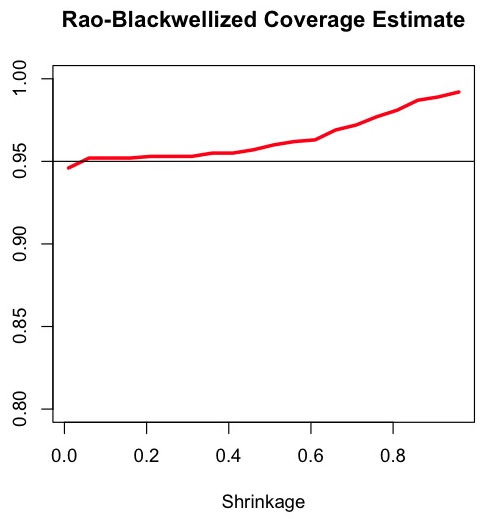
\includegraphics[width = 5.5cm]{baseball4.png}
%\end{center}
%\end{figure}

%We drew \code{cov.save} on \code{shr}, conneting dots. It shows that the estimated shrinkages are at least 0.946 on the tried range of true shrinkage values, slightly deviating from the definition of 95\% confidence interval. Note that even this result does not guarantee good repeated sampling property because $\beta$ was fixed. But, this result can definitely be an encouraging sign for our model's good repeated sampling property. 

%The reason we tried true shrinkage values between 0.01 and 0.99 is that no shriankge ($\equiv r / (r + n_{j}))$, corresponding to $r=0$, makes parameters of the second-level distribution 0 (see (8)), and full shrinkage corresponds to $r=\infty$ that we cannot designate as an argument of \code{coverage} function.

\section[Discussion]{Discussion}
\pkg{Rgbp} is an R package for estimating and validating two-level Gaussian, Poisson and Binomial hierarchical models. The package aims to provide a procedure that is computationally efficient with good frequency properties and includes ``method checking'' functionality to examine repeated sampling properties and test that the method is valid at given hyper-parameter values.

As an alternative to other derivative based estimation methods such as MLE and REML \pkg{Rgbp} provides point and interval estimates of true parameters using the ADM framework. Using the ADM framework in conjunction with the specified choice of priors safeguards from cases of overshrinkage and undercoverage that the aforementioned methods suffer from.

%In addition to good frequency properties Bayesians will be able to use the package to see the results from a non-informative reference point. This allows the user to examine whether it is worth to implement a full Bayesian model (which is often more time consuming). 

A benefit of \pkg{Rgbp} is that it produces non-random output, unlike most MCMC methods,  and so results can easily be reproduced and compared across studies. In addition to being a standalone analysis tool the package can be used as an aid or a tool in a broader estimation procedure. Such as being used

\begin{enumerate}
\item to initialize an MCMC to speed up time to convergence.
\item to check the validity of the code of an MCMC program.
\item as evaluated modules in object-oriented programming.
\item for preliminary data analyses.
\item as a demo that a particular prior gives adequate coverage.
\item for frequentist procedure checking.
\item for model checking.
\item to see if there is any reason to develop and use a more precise shrinkage method.

%%these are more ADM than RGBP
%%\item for computational speed.
%%\item as an envelope for accept-reject and importance sampling possibly leading to higher acceptance ratios than standard envelopes. 
\end{enumerate}

\pkg{Rgbp} provides a computationally efficient estimation procedure for Gaussian, Poisson and Binomial hierarchical models. An extension to Rgbp, that is underway, is to include functionality for fitting Gamma hierarchical models. 

\section[acknowledgments]{Acknowledgments}
The authors thank Professor Cindy Christiansen, Professor Phil Everson and the 2012 class of Harvard's Stat 324r: Parametric Statistical Inference and Modeling for their valuable inputs.

\bibliography{bibliography}

\end{document}
